\documentclass[12pt, twoside]{article}
\usepackage[top=4.3cm, bottom=5.7cm, left = 3.74cm, right = 3.75cm]{geometry}
\usepackage{times}
\usepackage{authblk}
\usepackage{graphicx} 
\usepackage{amsmath}
\usepackage{amssymb}
\usepackage{amsthm}
\usepackage{cite}
\usepackage{graphicx}
\usepackage{epstopdf}
\usepackage{amssymb}
\usepackage{chemfig}
\usepackage{centernot} 
\usepackage[labelsep=space]{caption}
\usepackage{float}
\renewcommand{\figurename}{Fig.}


\begin{document}
	\begin{center}
	\begin{huge}
	
	\textbf{Human-computer interfaces for various robotic platforms}
	\end{huge}
	
	\begin{large}
		Cătălina SÎRBU$^1$
	\end{large}
	
	
	\small {$^1$Politehnica University of Bucharest, Faculty of Electronics, Telecommunications and Technology of Information, Bucharest, Romania}
	
	\texttt {Email: catalinageorgiana9428@gmail.com}
	
	\textbf{Key-words:} Human-Computer Interface; Human-Computer Interaction; Human-Machine Interaction; Graphical User Interface; Behavioral Sciences; Gesture Control; Automatic Speechreading; Human-controlled surgery robot; Assistant driver
	\end{center}

\section{Introduction}

An interface is a surface that forms a common boundary between two things or a point of interaction between two components or systems. An example of an interface is someone using the controls on a washing machine to tell the machine how to function.

Human-Computer interaction (HCI) represents research in the design and the use of computer technology, which focuses on the interfaces between people (users) and computers.

HCI can be used in all disciplines wherever there is a possibility of the computer installation. Some of the areas where HCI can be implemented with distinctive importance are computer science, autonomous driving, psychology, and industrial design. 

For a Human–Machine Interface, the flow will be outlined in terms of information, control, and decision theories. In these terms, these processes can be characterized within the context of the information-processing requirements of the task being performed: namely, the observability and controllability of the state of the task being conducted using the interface.

\section{Summaries of the ‘selected papers’}
\subsection{Myo Gesture Control Armband for Medical Applications - Mahmoud Abduo, Matthias Galster\cite{1}}
The Myo Gesture Control Armband (Fig. 1) reads the electrical activity of the muscles and the motion of the arm. For disabled people with mobility problems, hand gesture-based HCIs should be specifically designed.

This armband it’s made of 8 medical grade stainless steel EMG sensors for presentation and observation of the electric potential of the muscles as a result of muscle activation. Using a gyroscope, an accelerometer, and a magnetometer, the orientation and movement of the patient's arm (roll, pitch, and yaw) can be determined.

Although it was created for use in gaming systems and control applications in mobile phones and computers, this wristband has been also exploited and used in the field of medicine and healthcare to improve the public health care system. The human gestures will allow gathering a huge amount of data and a series of EMG lines which can be analysed to detect medical abnormalities and hand movements.
\begin{figure}[!h]
    \centering
    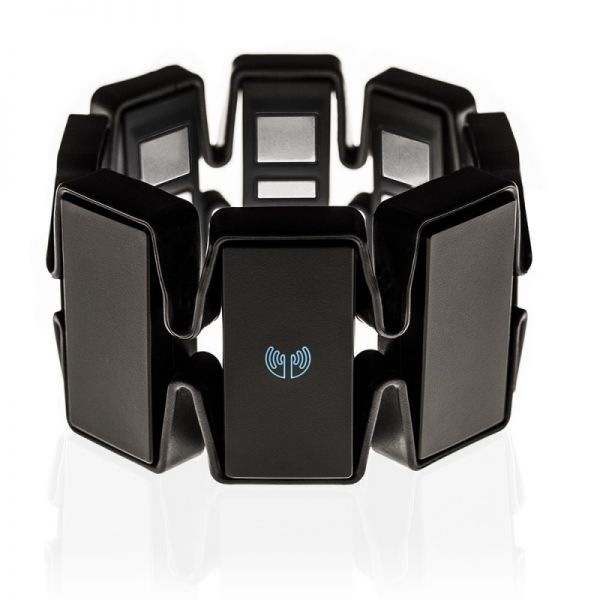
\includegraphics[width=0.4\linewidth]{photo1}
    \caption{Myo Armband}
\end{figure}

\subsection{Emotion-Sensitive Human-Computer Interfaces - Thomas S. Polzin And Alexander Waibel\cite{2}}
The integration of information of the user's expressed emotion into a dialog system becomes an essential part in building effective human-computer interfaces.  The authors modeled emotion-specific word choice information by computing the probability of a certain word given the previous word and the speaker's expressed emotion. The idea behind computing these probabilities is that certain word combinations are more probable for the expression of certain emotions.

In this study, they analysed both verbal and non-verbal information such as prosody (the rhythm, stress, and intonation of speech) and spectral (voice quality, clarity, or pleasantness).

The training and testing part was based on several thousands of sad, angry, and neutral speech segments from English movies. Regardless of the three categories of emotions, the experiment managed to achieve an accuracy of 60\% on average, but people managed to classify even more accurately than the program. 

An adequate emotion-sensitive human-computer interface has to meet at least two requirements: detection of the user’s expressed emotion and adjustment of system behavior with respect to the expressed emotion. In the future, it is also intended to add more categories such as speaking rate or stress distribution.

\subsection{Human-Computer Interfaces For Interaction With Surgical Tools In Robotic Surgery - C. Staub, S. Can, B. Jensen, And A. Knoll, S. Kohlbecher\cite{3}}
Researchers investigate methods that aim to make robot-assisted systems more intelligent, in particular targeting the improvement of both patient safety and operating time.

The ARAMIS system was created in order to satisfy the need for the execution of autonomous tasks in minimally invasive surgery and increase the operation complexity of telepresence systems. In the ARAMIS system, four ceiling-mounted manipulators are tele-operated via a master console. The robots can either be equipped with a surgical tool or an endoscopic stereo camera. For a high immersion, the surgeon is located in front of a stereo display and operates the system with haptic devices. The surgeon has a certain degree of mobility in front of the screen, instead of requiring a fixed head position at the master console because a head-mounted eye-tracking solution was implemented.

The eye tracker consists of one infrared camera which is mounted laterally to a goggle frame. The eye is illuminated by infrared LEDs positioned in the goggle frame which allows for a clean signal independent of the ambient lighting conditions. The camera image is transmitted via FireWire to a Mac, where image processing algorithms are used to detect the exact dark pupil position. An improvement for fixation accuracy can be an extension of the tracking system to two cameras, one for each eye.

\subsection{Automatic Speechreading With Applications To Human-Computer Interfaces - Xiaozheng Zhang, Charles C. Broun, Russell M. Mersereau, Mark A. Clements\cite{4}}
Natural means of communicating between humans and computers using speech instead of a mouse and keyboard provide an attractive alternative for HCI. Much research has been carried out in automatic speech recognition (ASR) and mainstream speech recognition has focused almost exclusively on the acoustic signal.

This study focuses on the recognition of the lip inner contour and the visibility of the tongue and teeth. In order to enable automatic speech and speaker recognition, the algorithm creates a region of interest around the mouth and segments the lip from its surrounding by making use of both color and edge information. The experiment was made using hue/saturation and motion information from a color video sequence of a speaker’s frontal view and involved discrimination of a set of 78 isolated words spoken by ten subjects.

It was found that this method achieved an increased accuracy when compared with previous studies that use only lip outer contour features.

\subsection{Design Of Human-Computer Interfaces For Highly Automated Vehicles In The Eu-Project Haveit - Frank Flemisch, Anna Schieben, Nadja Schoemig, Matthias Strauss, Stefan Lueke, And Anna Heyden\cite{5}}
Every day new forms of assistance and automation in vehicles open up the potential to increase safety and improve comfort. Research organizations, suppliers, car and truck manufacturers explore highly automated driving applications, where the automation can take over substantial parts of the driving task while the driver is still in action. There are discrete levels of automation that can be distinguished from each other from driver only to fully autonomous.

The identification of driver negligence is based on the outputs of the component which is able to detect different levels of drowsiness and distraction by means of direct (camera-based) and indirect (driving performance-based) measures. The system may initially start with a low urgency information message that encourages the driver to take a break in case of exhaustion or get back on the road in case of distraction. If the driver does not react, a higher level of urgency is reached, in which the driver's assistant intervenes and the vehicle should be brought to a safe stop. An example of this situation it is exposed in Fig.2.

In this research, highly automated driving was explored. The human-machine interfacing principles were iteratively developed in a design, implementation, and test approach, balancing human and technical factors, and base and applied research questions. Interactions schemes like the assistance and automation scale or interlocked transitions were defined, implemented and tested in simulators and test vehicles. While the research on the human-computer interaction of highly automated driving is still growing, the user acceptance gained in HAVEit is already quite promising.

\begin{figure}[!h]
    \centering
    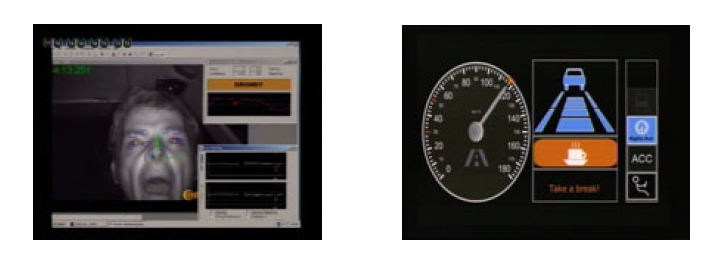
\includegraphics[width=0.7\linewidth]{photo2}
    \caption{Driver yawning from fatigue and Driver Assisted System with an informative message}
\end{figure}

\section{Conclusions}
I noticed that the experiments in the articles are based on both software and hardware development and that there are many areas where human-computer interfaces have been making their way since many years ago.

According to the approach to cognitive science, perception is essentially a proficient engagement with the world. Learning how to engage via a human-computer interface (HCI) can therefore be taken as an instance of developing a new mode of experience.

A consideration in studying or designing HCI is that user interface technology changes rapidly, offering new interaction possibilities to which previous research findings may not apply. Finally, user preferences change as they gradually master new interfaces.

\begin{thebibliography}{24}

\bibitem{1}	Mahmoud \uppercase{Abduo}, Matthias \uppercase{Galster}, \textit{Myo Gesture Control Armband for Medical Applications}, Department of Computer Science and Software Engineering, University of Canterbury, 2015.

\bibitem{2}	Thomas S. \uppercase{Polzin}, Alexander \uppercase{Waibel}, \textit{Emotion-Sensitive Human-Computer Interfaces}, Speech and Emotion, Newcastle, Northern Ireland, September 5-7, 2000.

\bibitem{3}	C. \uppercase{Staub}, S. \uppercase{Can}, B. \uppercase{Jensen}, B. \uppercase{Knoll}, S. \uppercase{Kohlbecher},\textit{Human-Computer Interfaces For Interaction With Surgical Tools In Robotic Surgery}, The Fourth IEEE RAS/EMBS International Conference on Biomedical Robotics and Biomechatronics, Roma, Italy. June 24-27, 2012.

\bibitem{4}	Xiaozheng  \uppercase{Zhang}, Charles C. \uppercase{Broun}, Russell M. \uppercase{Mersereau}, Mark A \uppercase{Clements}, S. \uppercase{Kohlbecher},\textit{Automatic Speechreading With Applications To Human-Computer Interfaces}, EURASIP J. Adv. Signal Process, 2002.

\bibitem{5}	Frank  \uppercase{Flemisch}, Anna  \uppercase{Schieben}, Nadja \uppercase{Schoemig}, Matthias \uppercase{Strauss}, Stefan \uppercase{Lueke}, Anna  \uppercase{Heyden}, \textit{Design Of Human-Computer Interfaces For Highly Automated Vehicles In The Eu-Project Haveit}, Universal Access in Human-Computer Interaction. Context Diversity. UAHCI 2011. Lecture Notes in Computer Science, vol 6767. Springer, Berlin, Heidelberg, 2011.

\end{thebibliography}

\end{document}